\section{JSON Web Signature}

In the former chapter MACs and digital signatures were discussed. One way to apply them in MQTT to provide integrity is by using them with the "JSON Web Signature"-framework hereinafter examined. 

\subsection{Definition of JSON Web Signature}
The
"JSON Web Signature (JWS) represents content secured with digital signatures or Message Authentication Codes (MACs) using JSON-based  data structures" \cite{rfc7515}.
A valid JWS consists of the following components : The JOSE Header, the JWS Payload and the JWS Signature \cite{rfc7515}.\newline
\subsection{The Components}
The \textbf{JOSE Header} (JSON Object Signing and Encryption ) is a JSON object consisting of a set of Header Parameters, which defines the parameters and the cryptographic operations used to secure the JWS Payload \cite{rfc7515}. There are two types of headers, which combined form the JOSE Header: \begin{center} The \textbf{JWS Protected Header} and the \textbf{JWS Unprotected Header}.
\end{center}
Both are JSON objects, but the difference is the JWS Protected Header contains the integrity protected Header Parameters whereas the JWS Unprotected Header contains the integrity unprotected parameters.\newline
An example for a Header Parameter is the "alg" (algorithm) Header Parameter which must be present in the JOSE Header. This parameter "identifies the cryptographic algorithm used to secure the JWS. The JWS Signature is not valid if the "alg" value does not represent a supported algorithm or if there is no key for use with that algorithm associated with the party that digitally signed or MACed the content" \cite{rfc7515}.\newline \newline
The \textbf{JWS Payload} can be described as the "sequence of octets to be secured -- a.k.a. the message. It can be any arbitrary sequence of octets"\cite{rfc7515}.\newline
The claims in a JWT, encoded as a JSON object, are often used as the payload \cite{rfc7519}.\newline
Two examples for claim names, both not mandatory, but very useful, are "iss" and "exp". "The "iss" (issuer) identifies the principal that issued the JWT" \cite{rfc7519} and "the "exp" (expiration time) identifies when the JWT MUST NOT be accepted for processing "\cite{rfc7519}. \newline \newline
The \textbf{JWS Signature} "is the computation of a Mac or digital signature over the JWS Protected Header and the JWS Payload"\cite{rfc7515}.\newline 
\subsection{The serialization}
The JWS can be further characterized by its two serializations:\begin{center} The \textbf{JWS Compact Serialization} and the \textbf{JWS JSON Serialization}.\end{center}
In the JWS Compact Serialization the JWS is represented as a compact, URL-safe string \cite{rfc7515} and can be portrayed in the following form:
\begin{figure}
\centering
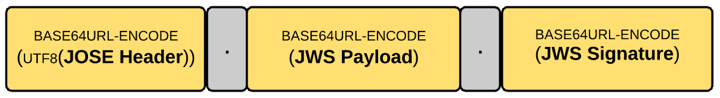
\includegraphics[width=10cm]{Pages/JWS/CompactSerialization.png}
\caption{JWS Compact Serialization}\cite{Compact}
\end{figure}

The dots are used to concatenate the components.
In this serialization, the JWS Protected Header is used as the JOSE Header. Therefore, no JWS Unprotected Header will be used.

In contrast to the JWS JSON Serialization, the JWS Compact Serialization provides no syntax for a JWS Unprotected Header and only supports one digital signature/MAC.
In the JWS JSON Serialization there are two related syntaxes: A flattered syntax, to secure content with only one MAC/digital signature and a fully general syntax, for securing with more than one MAC/digital signature \cite{rfc7515}. In this section, only the fully general syntax is treated. 
A JWS in the fully general JWS JSON Serialization "includes 2 top-level elements: payload and signatures (which is a JSON array), and three sub elements under each entry of the signatures array: protected, header and signature"\cite{Dummies}.
In each entry at least one of the values "protected" or "header" must be present to guarantee the "alg" Header Parameter is present \cite{rfc7515}.\newline
An example of this concept can be displayed as follows:\newline 
	\begin{figure}
\centering
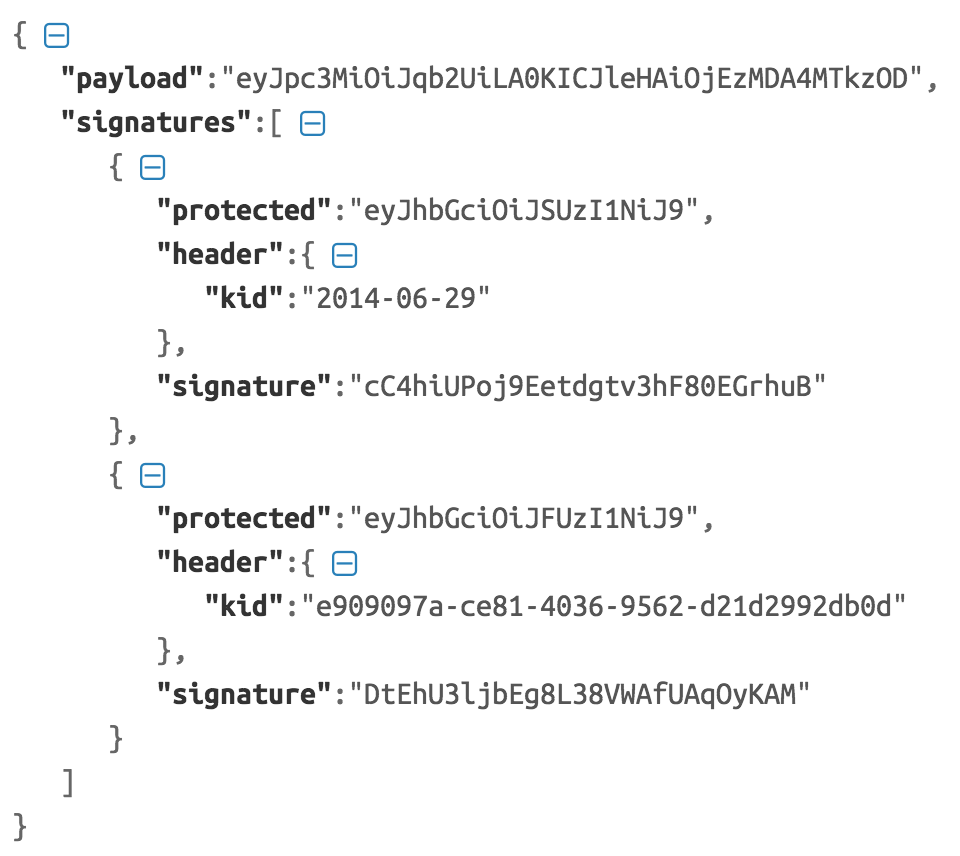
\includegraphics[width=8cm]{Pages/JWS/JSONSerialization.png}
\caption{JWS JSON Serialization} \cite{JSON}
\end{figure}
\subsection{The computation and validation }
For both types of serializations, the computation of a JWS is similar. To create a valid JWS the following steps have to be performed \cite{rfc7515}: 
\begin{enumerate} [leftmargin=1cm,rightmargin=1cm]\itemsep0.2em
\item Generate the desired content, which will be the payload of the JWS.
\item Compute the Base64Url-encoded payload. 
\item "Create the JOSE Header with the desired set of Header Parameter as a JSON object" \cite{rfc7515}.
\item Compute the UTF8 representation of the JWS Protected Header and base64url-encode it.
\item Create the signature by using the algorithm, defined in "alg",\newline over 
\begin{figure}
\centering
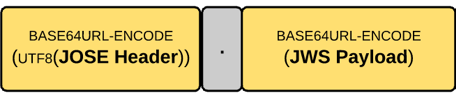
\includegraphics[width=8cm]{Pages/JWS/SigningInput.png}
\caption{JWS Signing Input}\cite{Compact} (Modified)
\end{figure}
, which is defined as the \textbf{JWS Signing Input}. If "alg" has the value "none", there will be no signature.
\item Compute the encoded signature by base64url-encode the JWS Signature .
\item For the JWS JSON Serialization the steps 3-6 have to be repeated for each MAC/digital signature defined in the JWS JOSE Header.
\item Compute the specific serialization output. For the structure look at the description of JWS Compact Serialization and JWS JSON Serialization.
\end{enumerate} 
After the computation the valid JWS could be placed in the payload of an MQTT message and sent to the intended receiver, where it should be validated.
As the computation of a JWS, the validation of a JWS is again similar for both types of serialization. It is important to note that if there are multiple signatures, like in the fully general JWS JSON Serialization,  it is application-specific how many and which JWS Signature must be validated successfully \cite{rfc7515}. However, at least one JWS Signature MUST be validated successfully.
To validate a JWS, the following steps have to be performed:\newline  
\begin{enumerate} [leftmargin=1cm, rightmargin=1cm] \itemsep0.3em
\item "Parse the JWS representation to extract the serialized values for the components of the JWS" \cite{rfc7515}. Look at the specific serialization for the components.
\item Decode the base64url-encoded JWS Protected Header.
\item Verify that the result of step 2 is a UTF8-encoded, valid JSON object.
\item For the JWS Compact Serialisation the JWS Protected header is used as the JOSE Header. For the JWS JSON Serialisation the JWS Protected Header Members and the JWS Unprotected Header Members combined build the JOSE Header.
\item Verify that all fields, which are required to be supported, are understood and can be processed by the implementation.

\item Decode the Base64Url-encoded JWS Payload.
\item Decode the Base64Url-encoded JWS Signature.
\item Validate if the JWS Signing input maced/digitally signed conformed the JWS Signature.
\item For the JWS JSON Serialisation the steps 4-8 have to be repeated for each MAC/digital signature defined in the JWS JOSE Header.
\item The JWS MUST be considered invalid if all validations in step 9 failed. (In the case of JWS Compact Serialization it is easy to indicate whether the JWS was validated successfully or not, by the result, whereas in the case of the JWS JSON serialization the result only indicates which validation was successfull and which not.)
\end{enumerate}
How precise a JWS can provide integrity depends on which and how much MACs/digital signatures are being used. If there is no algorithm, integrity cannot be guaranteed. 

\subsection{Input on MQTT packet}
To exemplify the impact of an JWS on a Mqtt packet. The hashfuction used is the same as in section ... to exemplify the difference between 
The JWS Compact Serialization is chosen for this example, because only one MAC will be used for the example
After following the steps for the computation in section 7.4 and u

Using the HS256 and the key ""


The valid JWS is: eyJhbGciOiJIUzI1NiJ9.aW50ZWdyaXR5IGNhbiBiZSBndWFyYW50ZWVkLCBpZiB5b3UgYXJlIGFibGUgdG8gcmVjYWxjdWxhdGUgdGhpcyBwYXJ0Og.eyJhbGciOiJIUzI1NiJ9.ZWViNGQxYmZhMzA0YWQwNzdiOGM5Y2U1ZWUwNmE5Nzc4MGYwNzZmNQ



\begin{table}[]
\centering
\begin{tabular}{lllllllllllllllll}
45 & 00 & 00 & 8d & 28 & c9 & 40 & 00 &  & 80 & 06 & ec & 47 & c0 & a8 & b2 & 02 \\
c0 & a8 & b2 & 06 & e6 & a4 & 07 & 5b &  & 8b & bf & b9 & 65 & fb & 88 & a4 & e7 \\
50 & 18 & 01 & 00 & 05 & b0 & 00 & 00 &  & 30 & 82 & 1a & 00 & 13 & 2f & 69 & 73 \\
2f & 69 & 74 & 2f & 6f & 66 & 2f & 69 &  & 6e & 74 & 65 & 67 & 72 & 69 & 74 & 79 \\
69 & 6e & 74 & 65 & 67 & 72 & 69 & 74 &  & 79 & 20 & 63 & 61 & 6e & 20 & 62 & 65 \\
20 & 67 & 75 & 61 & 72 & 61 & 6e & 74 &  & 65 & 65 & 64 & 2c & 20 & 69 & 66 & 20 \\
79 & 6f & 75 & 20 & 61 & 72 & 65 & 20 &  & 61 & 62 & 6c & 65 & 20 & 74 & 6f & 20 \\
72 & 65 & 63 & 61 & 6c & 63 & 75 & 6c &  & 61 & 74 & 65 & 20 & 74 & 68 & 69 & 73 \\
20 & 70 & 61 & 72 & 74 & 3a & 65 & 79 &  & 4a & 68 & 62 & 47 & 63 & 69 & 4f & 69 \\
4a & 49 & 55 & 7a & 49 & 31 & 4e & 69 &  & 4a & 39 & 2e & 61 & 57 & 35 & 30 & 5a \\
57 & 64 & 79 & 61 & 58 & 52 & 35 & 49 &  & 47 & 4e & 68 & 62 & 69 & 42 & 69 & 5a \\
53 & 42 & 6e & 64 & 57 & 46 & 79 & 59 &  & 57 & 35 & 30 & 5a & 57 & 56 & 6b & 4c \\
43 & 42 & 70 & 5a & 69 & 42 & 35 & 62 &  & 33 & 55 & 67 & 59 & 58 & 4a & 6c & 49 \\
47 & 46 & 69 & 62 & 47 & 55 & 67 & 64 &  & 47 & 38 & 67 & 63 & 6d & 56 & 6a & 59 \\
57 & 78 & 6a & 64 & 57 & 78 & 68 & 64 &  & 47 & 55 & 67 & 64 & 47 & 68 & 70 & 63 \\
79 & 42 & 77 & 59 & 58 & 4a & 30 & 4f &  & 67 & 2e & 65 & 79 & 4a & 68 & 62 & 47 \\
63 & 69 & 4f & 69 & 4a & 49 & 55 & 7a &  & 49 & 31 & 4e & 69 & 4a & 39 & 2e & 5a \\
57 & 56 & 69 & 4e & 47 & 51 & 78 & 59 &  & 6d & 5a & 68 & 4d & 7a & 41 & 30 & 59 \\
57 & 51 & 77 & 4e & 7a & 64 & 69 & 4f &  & 47 & 4d & 35 & 59 & 32 & 55 & 31 & 5a \\
57 & 55 & 77 & 4e & 6d & 45 & 35 & 4e &  & 7a & 63 & 34 & 4d & 47 & 59 & 77 & 4e \\
7a & 5a & 6d & 4e & 51
\end{tabular}
\caption{Basic packet with valid JWS}
\label{tab:my-table}
\end{table}
